\documentclass{article}
\usepackage{amsmath}
\usepackage{graphicx}
\usepackage{amssymb}
\usepackage{tikz}
\usepackage{xcolor}
\usepackage{tabularx}
\usepackage[letterpaper, margin=0.5in]{geometry}


\begin{document}
\begin{center}
	{\Huge EMCH367 --- Homework \#1}
\end{center}
Jacob C. Vaught, Completed 09-16-2024

\section*{Problem 1 (20pt)}
\textbf{True or False}
\begin{enumerate}
	\item Mathematical modeling of LTI system does not vary over time.\newline
	      \textcolor{blue}{LTI stands for Linear Time-Invariant. The ``Time-Invariant'' part means that the system's characteristics do not change over time, so its mathematical model remains constant.}
	\item Principle of superposition holds for linear system.\newline
	      \textcolor{blue}{The principle of superposition states that the response caused by two or more stimuli is the sum of the responses that would have been caused by each stimulus individually. This principle holds true for linear systems, meaning you can add up the individual effects to get the total effect.}
	\item Closed loop system does not need sensors.\newline
	      \textcolor{blue}{A closed-loop system uses feedback to control its output. This feedback usually comes from sensors that monitor the output. Without sensors, the system cannot adjust its behavior based on the output, making effective control impossible.}
	\item Complementary solution of spring-damper system is given as an exponential function.\newline
	      \textcolor{blue}{In a spring-damper system, which typically leads to a differential equation, the complementary (or homogeneous) solution often involves exponential terms. These solutions describe how the system's natural response (like oscillations) decays or grows over time.}
	\item Mass-spring-damper system is a second order system.\newline
	      \textcolor{blue}{A mass-spring-damper system generally leads to a second-order differential equation because it involves terms that describe acceleration (which is the second derivative of position).}
	\item Laplace transformation is a nonlinear operator.\newline
	      \textcolor{blue}{The Laplace transform is a linear operator. This means if you apply the Laplace transform to a linear combination of functions, the result is the same linear combination of the Laplace transforms of those functions.}
	\item Laplace transform of a unit step function is 1/s.\newline
	      \textcolor{blue}{The Laplace transform of the unit step function \( u(t) \) is \( \frac{1}{s} \) due to the theory of Laplace transforms used in solving differential equations and analyzing systems.}
	\item Laplace transform of differentiation does not need initial conditions.\newline
	      \textcolor{blue}{When applying the Laplace transform to a derivative, initial conditions are needed to solve the transformation completely. These conditions help in determining constants that arise during the transformation.}
	\item Final value theorem, $\lim_{t \to \infty} f(t) = \lim_{s \to 0} sF(s)$, is true for any $f(t)$.\newline
	      \textcolor{blue}{The final value theorem holds only if all poles of \( sF(s) \) are in the left half of the s-plane except possibly a simple pole at s=0. If \( f(t) \) does not meet these conditions, the theorem does not apply.}
	\item Transfer function is the Laplace transform of the output to the Laplace transform of the input.\newline
	      \textcolor{blue}{The transfer function of a system is defined as the Laplace transform of the system's output divided by the Laplace transform of the input, assuming zero initial conditions. This function characterizes the system's response to various inputs.}
	      	      
\end{enumerate}
\begin{center}
	\noindent % Ensures the table spans the text width starting from the left margin
	\begin{tabularx}{\textwidth}{|*{10}{X|}} % Creates 10 equal-width columns that fill the page
		\hline
		Q1 & Q2 & Q3 & Q4 & Q5 & Q6 & Q7 & Q8 & Q9 & Q10 \\ \hline
		T  & T  & F  & T  & T  & F  & T  & F  & F  & T   \\ 
		\hline
	\end{tabularx}
\end{center}


\newpage
\section*{Problem 2 (20pt)}
\subsection*{Transformation and Transfer Function}
\begin{enumerate}
	\item[(a)] \textbf{Find the Laplace transformation of the following function:}
\end{enumerate}   
\[
	f(t) = 
	\begin{cases} 
		0,                 & t < 0    \\
		\sin(wt + \theta), & t \geq 0 
	\end{cases}
\]
where \( \theta \in \mathbb{R} \) is a constant.

\noindent The function can be rewritten using the angle sum identity:
\textcolor{blue}{\[
	\sin(wt + \theta) = \sin(wt)\cos(\theta) + \cos(wt)\sin(\theta)
\]}
Applying the Laplace transform to the trigonometric functions and considering that the function is zero for \( t < 0 \), we obtain:
\textcolor{blue}{\[
	\mathcal{L}\{\sin(wt)\} = \frac{w}{s^2 + w^2}, \quad \mathcal{L}\{\cos(wt)\} = \frac{s}{s^2 + w^2}
\]}
Therefore, the Laplace transform of \( f(t) \) is:
\textcolor{blue}{\[
	\boxed{\mathcal{L}\{f(t)\} = \cos(\theta) \mathcal{L}\{\sin(wt)\} + \sin(\theta) \mathcal{L}\{\cos(wt)\}
		= \cos(\theta) \frac{w}{s^2 + w^2} + \sin(\theta) \frac{s}{s^2 + w^2}
		= \frac{s \sin(\theta) + w \cos(\theta)}{s^2 + w^2}}
\]}
This represents the Laplace transform of the function \( f(t) \) for \( t \geq 0 \) with zero otherwise, incorporating the phase shift \( \theta \).
\newpage
\begin{enumerate}
	\item[(b)] \textbf{Find the Laplace transformation of $f(t)$ given in the figure.}
\end{enumerate}
	      
\begin{center}
	\begin{tikzpicture}
		% Draw axes
		\draw[thick,->] (-1,0) -- (4,0) node[anchor=north west] {$t$};
		\draw[thick,->] (0,-4) -- (0,4) node[anchor=south east] {$f(t)$};
			      		
		% Draw the rectangles
		\draw[thick] (0,3) -- (1.5,3) -- (1.5,-3) -- (3,-3) -- (3,0);
			      		
		% Add labels
		\node at (-0.3, 3) {$\frac{1}{a^2}$};
		\node at (-0.5, -3) {$-\frac{1}{a^2}$};
		\node at (1.25, 0.25) {$a$};
		\node at (3.25, 0.25) {$2a$};
			      		    
		% Draw small ticks on axes
		\draw (1.5, 0.1) -- (1.5, -0.1);
		\draw (3, 0.1) -- (3, -0.1);
	\end{tikzpicture}
\end{center}
The function \( f(t) \) is described by:
\[
	\textcolor{blue}{f(t) = \begin{cases} 
		\frac{1}{a^2} & \text{for } 0 \leq t < a \\
		-\frac{1}{a^2} & \text{for } a \leq t < 2a \\
		0 & \text{otherwise}
		\end{cases}}
\]
Applying the Laplace transform to each segment:
\[
	\textcolor{blue}{F(s) = \frac{1}{a^2} \left( \mathcal{L}\{u(t)\} - \mathcal{L}\{u(t-a)\} - \mathcal{L}\{u(t-a)\} + \mathcal{L}\{u(t-2a)\} \right)}
\]
Where:
\begin{itemize}
	\item \(\textcolor{blue}{\mathcal{L}\{u(t)\} = \frac{1}{s}}\) (Laplace transform of the unit step function).
	\item \(\textcolor{blue}{\mathcal{L}\{u(t-a)\} = e^{-as}/s}\) (Laplace transform of the unit step function shifted by \( a \)).
\end{itemize}
Simplifying the expression:
\[
	\textcolor{blue}{F(s) = \frac{1}{a^2} \left( \frac{1}{s} - \frac{e^{-as}}{s} - \frac{e^{-as}}{s} + \frac{e^{-2as}}{s} \right)}
\]
\[
	\textcolor{blue}{\boxed{F(s) = \frac{1}{a^2 s} \left( 1 - 2e^{-as} + e^{-2as} \right)}}
\]
This represents the Laplace transform of \( f(t) \), showing how the function transitions between positive and negative values over the intervals from 0 to \( a \) and from \( a \) to \( 2a \).


\newpage
\section*{Problem 3 (20pt)}
\begin{enumerate}
	\item[(a)] \textbf{Find the inverse Laplace transformation of the following function:}
\end{enumerate}

\[
	X(s) = \frac{1}{s(s+1)(s+2)(s+3)}
\]
First, perform partial fraction decomposition. We assume:
\[
	\textcolor{blue}{\frac{1}{s(s+1)(s+2)(s+3)} = \frac{A}{s} + \frac{B}{s+1} + \frac{C}{s+2} + \frac{D}{s+3}}
\]
To find the coefficients, multiply through by the denominator and equate to 1:
       
\[
	\textcolor{blue}{1 = A(s+1)(s+2)(s+3) + B(s)(s+2)(s+3) + C(s)(s+1)(s+3) + D(s)(s+1)(s+2)}
\]
Setting specific values for \(s\) to simplify the equations:

\textcolor{blue}{\begin{itemize}
	\item \(s = 0\), then \(1 = A(1)(2)(3)\), thus \(A = \frac{1}{6}\)
	\item \(s = -1\), then \(1 = B(-1)(1)(2)\), thus \(B = -\frac{1}{2}\)
	\item \(s = -2\), then \(1 = C(-2)(-1)(1)\), thus \(C = \frac{1}{2}\)
	\item \(s = -3\), then \(1 = D(-3)(-2)(-1)\), thus \(D = -\frac{1}{6}\)
	\end{itemize}}
\noindent The partial fractions thus are:

\[
	\textcolor{blue}{\frac{1}{s(s+1)(s+2)(s+3)} = \frac{1}{6s} - \frac{1}{2(s+1)} + \frac{1}{2(s+2)} - \frac{1}{6(s+3)}}
\]
Applying the inverse Laplace transform to each term:
\[
	\textcolor{blue}{\mathcal{L}^{-1}\left\{\frac{1}{6s} - \frac{1}{2(s+1)} + \frac{1}{2(s+2)} - \frac{1}{6(s+3)}\right\} = \frac{1}{6} - \frac{1}{2}e^{-t} + \frac{1}{2}e^{-2t} - \frac{1}{6}e^{-3t}}
\]
Thus, the inverse Laplace transform of \( X(s) \) is:
\[
	\textcolor{blue}{\boxed{x(t) = \frac{1}{6} - \frac{1}{2}e^{-t} + \frac{1}{2}e^{-2t} - \frac{1}{6}e^{-3t}, \quad t \geq 0}}
\]
\newpage
\begin{enumerate}
	\item[(b)] \textbf{Find the inverse Laplace transformation of the following function:}
\end{enumerate}
\[
	X(s) = \frac{1}{s^2(s+1)^2}
\]
We assume the decomposition:
\[
	\textcolor{blue}{\frac{1}{s^2 (s + 1)^2} = \frac{A}{s} + \frac{B}{s^2} + \frac{C}{s+1} + \frac{D}{(s+1)^2}}
\]
Multiply through by \(s^2 (s + 1)^2\) to eliminate the denominators:
\[
	\textcolor{blue}{1 = A s (s + 1)^2 + B (s + 1)^2 + C s^2 (s + 1) + D s^2}
\]
Expand and combine like terms:
\[
	\textcolor{blue}{1 = (A + C)s^3 + (2A + B + C + D)s^2 + (A + 2B)s + B}
\]
Solve the system of equations for coefficients:
\textcolor{blue}{\begin{itemize}
	\item \(s^3\) term: \(A + C = 0\)
	\item \(s^2\) term: \(2A + B + C + D = 0\)
	\item \(s^1\) term: \(A + 2B = 0\)
	\item Constant term: \(B = 1\)
	\end{itemize}}
From \(A + 2B = 0\):
\[
	\textcolor{blue}{A = -2}
\]
From \(A + C = 0\):
\[
	\textcolor{blue}{C = 2}
\]
Plugging in \(A, B, C\), and \(D = 1\) into the \(s^2\) term:
\[
	\textcolor{blue}{2(-2) + 1 + 2 + 1 = 0}
\]
The partial fractions are:
\[
	\textcolor{blue}{\frac{-2}{s} + \frac{1}{s^2} + \frac{2}{s+1} + \frac{1}{(s+1)^2}}
\]
The inverse Laplace transforms are straightforward:
\[
	\textcolor{blue}{\mathcal{L}^{-1}\left\{\frac{-2}{s}\right\} = -2}
\]
\[
	\textcolor{blue}{\mathcal{L}^{-1}\left\{\frac{1}{s^2}\right\} = t}
\]
\[
	\textcolor{blue}{\mathcal{L}^{-1}\left\{\frac{2}{s+1}\right\} = 2e^{-t}}
\]
\[
	\textcolor{blue}{\mathcal{L}^{-1}\left\{\frac{1}{(s+1)^2}\right\} = te^{-t}}
\]
Combining these gives the time-domain solution:
\[
	\textcolor{blue}{\boxed{x(t) = -2 + t + 2e^{-t} + te^{-t}}}
\]
\newpage
\section*{Problem 4 (20pt)}

\begin{center}
	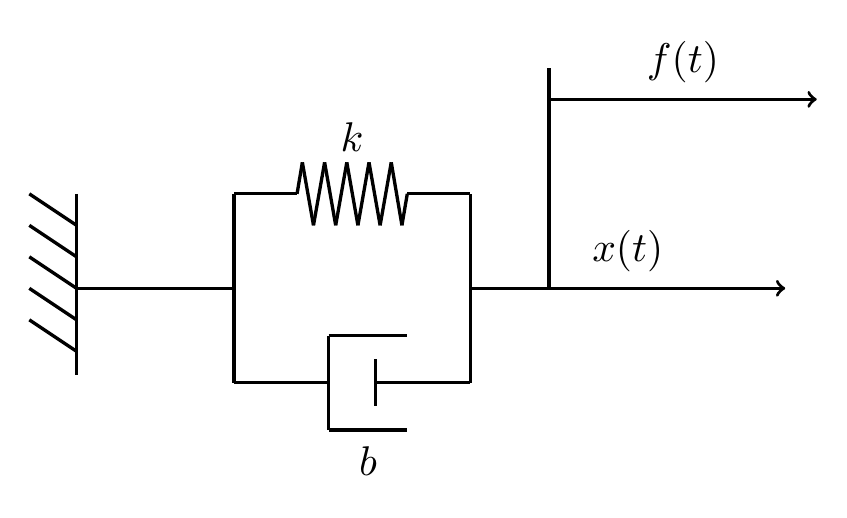
\begin{tikzpicture}[scale=0.4]
		% Multiple line segments with coordinates adjusted and line width increased
		\draw[line width=1.2pt] (0,6) -- (1.5,5);  % From (0,6) to (1.5,5)
		\draw[line width=1.2pt] (0,5) -- (1.5,4);  % From (0,5) to (1.5,4)
		\draw[line width=1.2pt] (0,4) -- (1.5,3);  % From (0,4) to (1.5,3)
		\draw[line width=1.2pt] (0,3) -- (1.5,2);  % From (0,3) to (1.5,2)
		\draw[line width=1.2pt] (0,2) -- (1.5,1);  % From (0,2) to (1.5,1)
				
		% Vertical line with coordinates adjusted and line width increased
		\draw[line width=1.2pt] (1.5,6) -- (1.5,0.25);  % Vertical line from (1.5,6) to (1.5,0.25)
				
		% Horizontal line with coordinates adjusted and line width increased
		\draw[line width=1.2pt] (1.5,3) -- (6.5,3);  % Horizontal line from (1.5,3) to (6.5,3)
		\draw[line width=1.2pt] (6.5,6) -- (6.5,0);
				    
		% Horizontal lines and line width increased
		\draw[line width=1.2pt] (6.5,0) -- (9.5,0);
		\draw[line width=1.2pt] (6.5,6) -- (8.5,6);
				
		% Vertical line and line width increased
		\draw[line width=1.2pt] (9.5,-1.5) -- (9.5,1.5);
				
		% Additional horizontal lines at -1.5 and 1.5 y-coordinates and line width increased
		\draw[line width=1.2pt] (9.5,-1.5) -- (12,-1.5);
		\draw[line width=1.2pt] (9.5,1.5) -- (12,1.5);
				
		% Vertical line at x = 11, and horizontal through x = 11 and line width increased
		\draw[line width=1.2pt] (11,0.75) -- (11,-0.75);
		\draw[line width=1.2pt] (11,0) -- (14,0);
		\draw[line width=1.2pt] (14,0) -- (14, 6);
		\draw[line width=1.2pt] (14,6) -- (12, 6);
				
		% Initial shifts and settings
		\def\xShift{8.33}
		\def\yShift{6} % Shifting everything to start at y = 6 for the intersection
				    
		% Draw the spring with adjustments and line width increased
		\draw[line width=1.2pt] (8.5, 6) -- (8.669, 7.0);
		\draw[line width=1.2pt] (8.669, 7) -- (9.022, 5.0);
		\draw[line width=1.2pt] (9.022, 5) -- (9.375, 7.0);
		\draw[line width=1.2pt] (9.375, 7) -- (9.727, 5.0);
		\draw[line width=1.2pt] (9.727, 5) -- (10.08, 7);
		\draw[line width=1.2pt] (10.08, 7) -- (10.433, 5.0);
		\draw[line width=1.2pt] (10.433, 5) -- (10.785, 7);
		\draw[line width=1.2pt] (10.785, 7) -- (11.138, 5.0);
		\draw[line width=1.2pt] (11.138, 5) -- (11.491, 7);
		\draw[line width=1.2pt] (11.491, 7) -- (11.83, 5);
		\draw[line width=1.2pt] (11.83, 5) -- (12,6);
				    
		% Draw arrow for displacement x(t) with larger text
		\draw[->, line width=1.2pt] (14,3) -- (24,3) node[midway, above, scale=1.5] {$x(t)$};
				    
		% Draw force arrow f(t) with larger text
		\draw[->, line width=1.2pt] (16.5,9) -- (25,9) node[midway, above, scale=1.5] {$f(t)$};
				    
		% Label for k (spring constant) with larger text
		\node[scale=1.5] at (10.25,7.8) {$k$};
				    
		% Label for b (damper constant) with larger text
		\node[scale=1.5] at (10.75,-2.5) {$b$};
				
		% Additional lines and adjustments with increased line width
		\draw[line width=1.2pt] (14,3) -- (14,0);  % Downward line from the end of x(t) arrow
		\draw[line width=1.2pt] (16.5, 3) -- (16.5,10);
	\end{tikzpicture}
\end{center}

\begin{enumerate}
	\item[(a)] \textbf{Draw free body diagram and find the force balance equation in ODE.}
\end{enumerate}
\begin{center}
	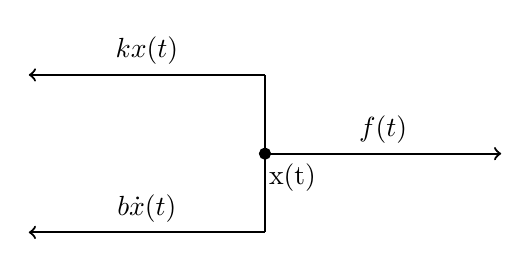
\begin{tikzpicture}
			      		    
		% Draw the point of interest
		\filldraw[black] (0,0) circle (2pt); % the point where forces are applied
			      		    
		% Draw the forces
		\draw[->, thick] (0,0) -- (3,0) node[midway, above] {$f(t)$}; % External force to the right
		\draw[<-, thick] (-3,1) -- (0,1) node[midway, above] {$kx(t)$}; % Spring force to the left
		\draw[<-, thick] (-3,-1) -- (0,-1) node[midway, above] {$b\dot{x}(t)$}; % Damping force to the left
		\draw (0,-1) -- (0,1);
			      		    
		% Add a label for the point
		\node[below] at (0.35,0) {x(t)};
			      		    
	\end{tikzpicture}
\end{center}
Following from the free-body diagram, the equation of motion for the system is:
\[
	\textcolor{blue}{k x(t) + b \dot{x}(t) = F(t)}
\]
\begin{enumerate}
	\item[(b)] \textbf{Derive the free vibration response.}
\end{enumerate}   
Starting with the equation of motion with \( F(t) = 0 \):
	      
\[
	\textcolor{blue}{b \dot{x}(t) + k x(t) = 0.}
\]
Dividing by \( k \) and letting \( T = \frac{b}{k} \):
	      
\[
	\textcolor{blue}{T \dot{x}(t) + x(t) = 0, \quad \text{or} \quad \dot{x}(t) + \frac{1}{T} x(t) = 0.}
\]
Using the integrating factor \( \mu(t) = e^{\frac{t}{T}} \):
	      
\[
	\textcolor{blue}{\frac{d}{dt} \left( e^{\frac{t}{T}} x(t) \right) = 0.}
\]
Integrating:
	      
\[
	\textcolor{blue}{e^{\frac{t}{T}} x(t) = C,}
\]
	      
\[
	\textcolor{blue}{\boxed{x(t) = C e^{-\frac{t}{T}}.}}
\]
	      
	          
\newpage
\begin{enumerate}
	\item[(c)] \textbf{Derive the forced vibration response with $f(t) = \frac{F(t)}{k} = \sin(wt)$ and $x(0) = 0$. (Hint: Define $T = \frac{b}{k}$, and consider $T$ and $w$ as constants.)}
\end{enumerate}
	      
	      
\noindent
\textcolor{black}{The following differential equation is given:}

\[
	\textcolor{blue}{T \dot{x}(t) + x(t) = f(t)}
\]

\noindent
\textcolor{black}{Taking the Laplace Transform of the above equation:}

\[
	\textcolor{blue}{T(sX(s) - x(0)) + X(s) = F(s)}
\]

\noindent
\textcolor{black}{With the initial condition \( x(0) = 0 \), the equation simplifies to:}

\[
	\textcolor{blue}{X(s) = \frac{1}{Ts + 1} F(s)}
\]

\noindent
\textcolor{black}{Given \( F(s) = \frac{\omega}{s^2 + \omega^2} \), we have:}

\[
	\textcolor{blue}{X(s) = \frac{\omega}{(s^2 + \omega^2)(Ts + 1)}}
\]

\noindent
\textcolor{black}{Using Partial Fraction Decomposition:}

\[
	\textcolor{blue}{\frac{\omega}{(Ts + 1)(s^2 + \omega^2)} = \frac{A}{Ts + 1} + \frac{Bs + C}{s^2 + \omega^2}}
\]

\noindent
\textcolor{black}{Multiplying both sides to clear the fractions:}

\[
	\textcolor{blue}{\omega = A(s^2 + \omega^2) + (Bs + C)(Ts + 1)}
\]

\noindent
\textcolor{black}{Grouping like terms:}

\[
	\textcolor{blue}{\omega = s^2(A + BT) + s(B + CT) + (C + A\omega^2)}
\]

\noindent
\textcolor{black}{Equating coefficients, we get:}

\[
	\textcolor{blue}{A + BT = 0, \quad B + CT = 0, \quad C + A\omega^2 = \omega}
\]

\noindent
\textcolor{black}{Writing this as a system of linear equations in matrix form:}

\[
	\textcolor{blue}{
		\begin{bmatrix}
			\omega^2 & 0 & 1 \\
			0        & 1 & T \\
			1        & T & 0 
		\end{bmatrix}
		\begin{bmatrix}
			A \\
			B \\
			C 
		\end{bmatrix}
		=
		\begin{bmatrix}
			\omega \\
			0      \\
			0      
		\end{bmatrix}
	}
\]

\noindent
\textcolor{black}{The solutions are:}

\[
	\textcolor{blue}{A = \frac{T^2 \omega}{T^2 \omega^2 + 1}, \quad B = \frac{-T\omega}{T^2 \omega^2 + 1}, \quad C = \frac{\omega}{T^2 \omega^2 + 1}}
\]

\noindent
\textcolor{black}{Taking the Inverse Laplace Transform yields the final solution:}

\[
	\textcolor{blue}{\boxed{\frac{T\omega e^{-\frac{t}{T}} - T\omega \cos(\omega t) + \sin(\omega t)}{T^2 \omega^2 + 1}}}
\]
\newpage
	      
\begin{enumerate}
	\item[(d)] \textbf{Let $k = 250$ N/m and $b = 400$ N$\cdot$s/m. Calculate time constant.}
\end{enumerate}
\noindent
\textcolor{black}{Given the values:}

\[
	\textcolor{blue}{k = 250 \, \text{N/m}, \quad b = 400 \, \text{N}\cdot\text{s/m}}
\]

\noindent
\textcolor{black}{The time constant \( T \) is defined as:}

\[
	\textcolor{blue}{T = \frac{b}{k}}
\]

\noindent
\textcolor{black}{Substituting the given values:}

\[
	\textcolor{blue}{T = \frac{400 \, \text{N}\cdot\text{s/m}}{250 \, \text{N/m}} = 1.6 \, \text{s}}
\]

\noindent
\textcolor{blue}{\boxed{\text{Thus, the time constant } T \text{ is } 1.6 \, \text{seconds}.}}


\newpage
\section*{Problem 5 (20pt)}

\begin{figure}[h]  % [h] means here, where the image will be placed
	\centering
	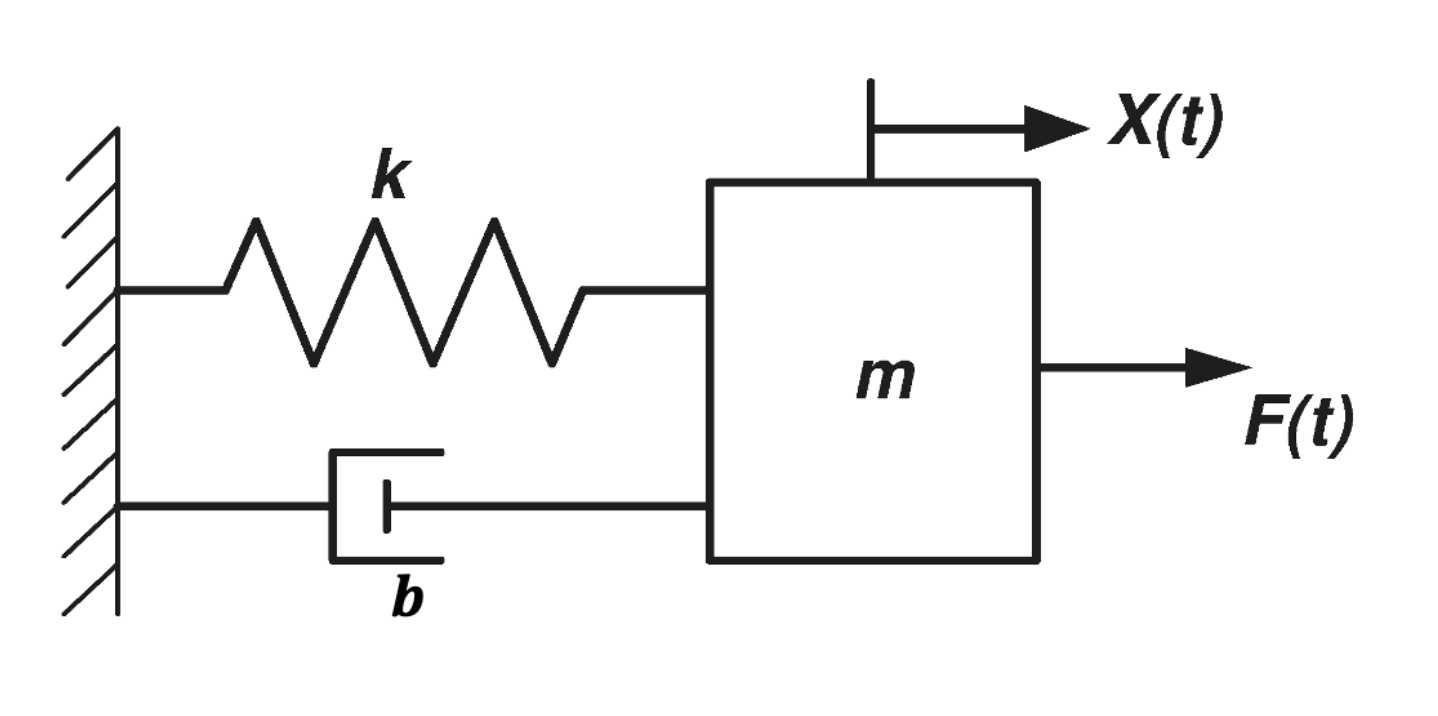
\includegraphics[width=0.5\textwidth]{prob2.png}  % Adjust width as needed
	\caption{Mass-Spring-Damper System}  % Optional, for captioning the image
	\label{fig:sample_image}  % Optional, for referencing the image in the text
\end{figure}

\begin{enumerate}
	\item[(a)] \textbf{Draw free body diagram and find the force balance equation in ODE.}
\end{enumerate}
\begin{center}
	\begin{tikzpicture}[scale=1.5]
			      		
		% Draw the vertical line through the circle
		\draw[thick] (0, -1.5) -- (0, 1.5);
			      		
		% Spring force with arrow and label
		\draw[->, thick] (0, 1) -- (-2.5, 1); % Arrow for spring force
		\node[above] at (-2, 1) {$-kx$}; % Label for spring force
			      		
		% Damper force with arrow and label
		\draw[->, thick] (0, -1) -- (-2.5, -1); % Arrow for damper force
		\node[below] at (-2, -1) {$-b\dot{x}$}; % Label for damper force
			      		
		% Draw a horizontal line to the right for F(t)
		\draw[thick, ->] (0, 0) -- (2, 0);
		\node[right] at (2, 0) {$F(t)$}; % Label for the applied force
			      		    
		% Draw the opaque circle at (0,0) with m in the center
		\filldraw[fill=white, thick] (0,0) circle (0.5);
		\node at (0, 0) {$m$};
	\end{tikzpicture}
\end{center}
\noindent  
The equation of motion for the mass-spring-damper system is given by:
	      
\[
	\textcolor{blue}{m\ddot{x} + b\dot{x} + kx = F(t),}
\]
\begin{enumerate}   
	\item[(b)] \textbf{What is the inverse Laplace transformation of $\frac{s}{(s+a)^2}$?}
\end{enumerate}
First, rewrite the function:
	      
\[
	\textcolor{blue}{\frac{s}{(s + a)^2} = \frac{(s + a) - a}{(s + a)^2} = \frac{s + a}{(s + a)^2} - \frac{a}{(s + a)^2}}.
\]
Next, split the expression into two simpler fractions:
	      
\[
	\textcolor{blue}{\frac{s}{(s + a)^2} = \frac{1}{s + a} - \frac{a}{(s + a)^2}}.
\]
Using standard inverse Laplace transforms:
	      
\[
	\textcolor{blue}{\mathcal{L}^{-1}\left\{\frac{1}{s + a}\right\} = e^{-at}} \quad \text{and} \quad \textcolor{blue}{\mathcal{L}^{-1}\left\{\frac{1}{(s + a)^2}\right\} = t e^{-at}}.
\]
Combining these results, we have:
	      
\[
	\textcolor{blue}{\mathcal{L}^{-1}\left\{\frac{s}{(s + a)^2}\right\} = e^{-at} - a t e^{-at}}.
\]
Simplifying, the final answer is:
	      
\[
	\textcolor{blue}{\boxed{\mathcal{L}^{-1}\left\{\frac{s}{(s + a)^2}\right\} = e^{-at} (1 - at)}}
\]
\newpage
\begin{enumerate}
	\item[(c)] \textbf{Find the free vibration response with $b^2 - 4mk = 0$ by using Laplace transformation. The initial conditions are given by $x(0) = x_0$ and $\dot{x}(0) = \dot{x}_0$.}
	      	      
\end{enumerate}
	      
\noindent
\textcolor{black}{Start with the equation of motion:}

\[
	\textcolor{blue}{m\ddot{x}(t) + b\dot{x}(t) + kx(t) = 0}
\]

\noindent
\textcolor{black}{This represents a mass-spring-damper system without external forcing, where \( m \) is the mass, \( b \) is the damping coefficient, and \( k \) is the spring constant.}

\noindent
\textcolor{black}{Apply the Laplace transform to the equation:}

\[
	\textcolor{blue}{s^2X(s) - sx(0) - \dot{x}(0) + \frac{b}{m} \left[sX(s) - x(0)\right] + \frac{k}{m}X(s) = 0}
\]

\noindent
\textcolor{black}{This equation transforms the time-domain differential equation into the \( s \)-domain.}

\noindent
\textcolor{black}{Combine like terms:}

\[
	\textcolor{blue}{X(s) \left( s^2 + \frac{b}{m}s + \frac{k}{m} \right) = \left(s + \frac{b}{m}\right)x(0) + \dot{x}(0)}
\]

\noindent
\textcolor{black}{The left side contains the characteristic polynomial, which describes the system's dynamics.}

\noindent
\textcolor{black}{Simplify the characteristic polynomial using the critical damping condition \(\textcolor{blue}{b^2 - 4mk = 0}\):}

\[
	\textcolor{blue}{s^2 + \frac{b}{m}s + \frac{k}{m}}
\]

\noindent
\textcolor{black}{Using \(\textcolor{blue}{\frac{k}{m} = \left(\frac{b}{2m}\right)^2}\), rewrite the polynomial as:}

\[
	\textcolor{blue}{s^2 + \frac{b}{m}s + \left(\frac{b}{2m}\right)^2 = \left(s + \frac{b}{2m}\right)^2}
\]

\noindent
\textcolor{black}{This shows that the system has repeated real roots, characteristic of critical damping.}

\noindent
\textcolor{black}{Substitute the simplified form back into the equation:}

\[
	\textcolor{blue}{X(s) \left( \left(s + \frac{b}{2m}\right)^2 \right) = \left(s + \frac{b}{m}\right)x(0) + \dot{x}(0)}
\]

\noindent
\textcolor{black}{Divide both sides by \(\left(s + \frac{b}{2m}\right)^2\):}

\[
	\textcolor{blue}{X(s) = \frac{\left(s + \frac{b}{m}\right)x(0) + \dot{x}(0)}{\left(s + \frac{b}{2m}\right)^2}}
\]

\noindent
\textcolor{black}{We need to find the time-domain response \( x(t) \).}

\noindent
\textcolor{black}{Rewrite \( X(s) \) in partial fractions:}

\[
	\textcolor{blue}{X(s) = \frac{\left(s + \frac{b}{m}\right)x_0 + \dot{x}_0}{\left(s + \frac{b}{2m}\right)^2}}
\]

\noindent
\textcolor{black}{Separate this expression into simpler terms:}

\[
	\textcolor{blue}{X(s) = \frac{x_0}{(s + \frac{b}{2m})^2} + \frac{\dot{x}_0 + \frac{b}{2m}x_0}{(s + \frac{b}{2m})^2}}
\]

\noindent
\textcolor{black}{Recognize the standard inverse Laplace forms:}

\[
	\textcolor{blue}{\mathcal{L}^{-1}\left\{\frac{1}{(s + \alpha)^n}\right\} = t^{n-1} \frac{e^{-\alpha t}}{(n-1)!}}
\]

\noindent
\textcolor{black}{Specifically, for our terms:}

\[
	\textcolor{blue}{\mathcal{L}^{-1}\left\{\frac{1}{(s + \frac{b}{2m})^2}\right\} = t e^{-\frac{b}{2m}t}}
\]

\noindent
\textcolor{black}{Applying the inverse Laplace transform to each term:}

\[
	\textcolor{blue}{x(t) = x_0 \cdot t e^{-\frac{b}{2m}t} + \left(\dot{x}_0 + \frac{b}{2m}x_0\right) \cdot t e^{-\frac{b}{2m}t}}
\]

\noindent
\textcolor{black}{Simplify to obtain the complete time-domain response:}

\[
	\textcolor{blue}{\boxed{x(t) = \left(x_0 + \left(\dot{x}_0 + \frac{b}{2m}x_0\right)t\right) e^{-\frac{b}{2m}t}}}
\]
	      
\noindent Interpretation of the solution:
	      
\begin{itemize}
	\item \(\textcolor{blue}{x_0 \cdot t e^{-\frac{b}{2m}t}}\): Represents the system's response due to initial displacement.
	\item \(\textcolor{blue}{\left(\dot{x}_0 + \frac{b}{2m}x_0\right) \cdot t e^{-\frac{b}{2m}t}}\): Represents the response due to initial velocity and damping.
	\item The combined response shows how the initial conditions affect the critically damped system, leading to non-oscillatory decay back to equilibrium.
\end{itemize}
\begin{enumerate}  
	\item[(d)] \textbf{Let $m = 10$ kg, $k = 160$ N/m, $b = 64$ N$\cdot$s/m, and $\omega = \pi/2$ s$^{-1}$. Calculate the damped frequency of the system.}
\end{enumerate}
\noindent
\textcolor{black}{The natural frequency is given by:}

\[
	\textcolor{blue}{\omega_n = \sqrt{\frac{k}{m}}}
\]

\noindent
\textcolor{black}{Substituting the given values:}

\[
	\textcolor{blue}{\omega_n = \sqrt{\frac{160}{10}} = \sqrt{16} = 4 \, \text{rad/s}}
\]

\noindent
\textcolor{black}{The damping ratio is defined as:}

\[
	\textcolor{blue}{\zeta = \frac{b}{2\sqrt{mk}}}
\]

\noindent
\textcolor{black}{Substituting the given values:}

\[
	\textcolor{blue}{\zeta = \frac{64}{2\sqrt{10 \times 160}} = \frac{64}{2 \times \sqrt{1600}} = \frac{64}{80} = 0.8}
\]

\noindent
\textcolor{black}{The damped natural frequency is given by:}

\[
	\textcolor{blue}{\omega_d = \omega_n \sqrt{1 - \zeta^2}}
\]

\noindent
\textcolor{black}{Substituting the calculated values:}

\[
	\textcolor{blue}{\omega_d = 4 \sqrt{1 - 0.8^2} = 4 \sqrt{1 - 0.64} = 4 \sqrt{0.36} = 4 \times 0.6 = 2.4 \, \text{rad/s}}
\]

\noindent
\textcolor{blue}{\boxed{\omega_d = 2.4 \, \text{rad/s}}}

\newpage
\section*{Bonus Problem (20pt)}
\textbf{Find the transfer function of the system given in Figure 4 wherein $x_i(t)$ is the input and $x_o(t)$ is the output. Assume that $x_i(0^-) = 0$ and $x_o(0^-) = 0$.}
% To insert an image
\begin{figure}[h]  % [h] means here, where the image will be placed
	\centering
	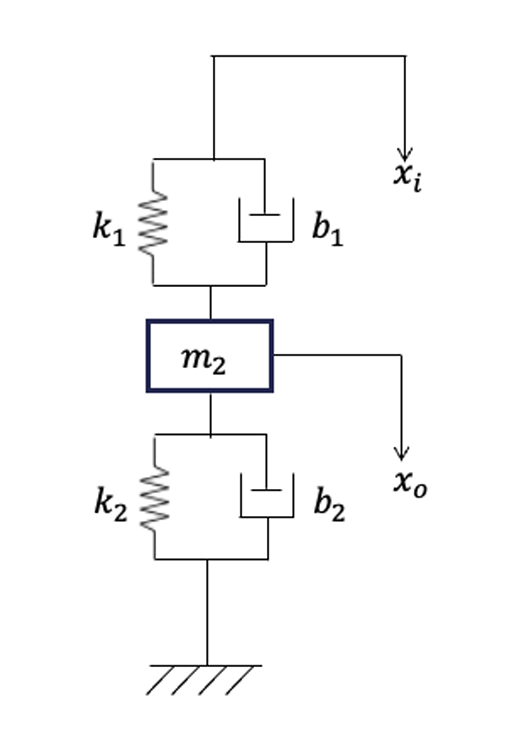
\includegraphics[width=0.2\textwidth]{bonus.png}  % Adjust width as needed
	\caption{Mass-Spring-Damper System}  % Optional, for captioning the image
	\label{fig:sample_image}  % Optional, for referencing the image in the text
\end{figure}
\newline
The free body diagram for the mass \( m_2 \) is shown below. It includes the forces from springs and dampers acting on the mass.

\begin{center}
	\begin{tikzpicture}[scale=0.4]
		% Draw the circle at (0,0) with radius 1 and label it as the mass m_2
		\draw[thick] (0,0) circle (1);
		\node at (0,0) {$m_2$};
				
		% Draw thick lines from (-5,0) to (-1,0) and (1,0) to (5,0)
		\draw[thick] (-5,0) -- (-1,0);
		\draw[thick] (1,0) -- (5,0);
				
		% Draw arrows with labels
		\draw[->] (-4,0) -- (-4,5); % Vertical arrow up from (-4,0)
		\node[left] at (-4,2.5) {$F_{k1} = k_1 (x_i - x_o)$};
				
		\draw[->] (-4.5,0) -- (-4.5,-5); % Vertical arrow down from (-4.5,0)
		\node[left] at (-4.5,-2.5) {$F_{k2} = k_2 x_o$};
				
		\draw[->] (4,0) -- (4,5); % Vertical arrow up from (4,0)
		\node[right] at (4,2.5) {$F_{b1} = b_1 (\dot{x}_i - \dot{x}_o)$};
				
		\draw[->] (4.5,0) -- (4.5,-5); % Vertical arrow down from (4.5,0)
		\node[right] at (4.5,-2.5) {$F_{b2} = b_2 \dot{x}_o$};
	\end{tikzpicture}
\end{center}

\noindent
\textcolor{black}{To find the transfer function, we take the forces acting on both sides of the mass \( m_2 \) and set them equal to the mass times its acceleration, \( m_2 \ddot{x}_o \), using Newton’s second law:}

\[
	\textcolor{blue}{m_2 \ddot{x}_o = k_1 (x_i - x_o) + b_1 (\dot{x}_i - \dot{x}_o) - k_2 x_o - b_2 \dot{x}_o}
\]

\noindent
\textcolor{black}{Combining and rearranging the terms, we get:}

\[
	\textcolor{blue}{m_2 \ddot{x}_o + (b_1 + b_2) \dot{x}_o + (k_1 + k_2) x_o = k_1 x_i + b_1 \dot{x}_i}
\]

\noindent
\textcolor{black}{Taking the Laplace transform of the above equation, assuming zero initial conditions:}

\[
	\textcolor{blue}{m_2 s^2 X_o(s) + (b_1 + b_2) s X_o(s) + (k_1 + k_2) X_o(s) = k_1 X_i(s) + b_1 s X_i(s)}
\]

\noindent
\textcolor{black}{Factoring out \( X_o(s) \):}

\[
	\textcolor{blue}{X_o(s) \left( m_2 s^2 + (b_1 + b_2) s + (k_1 + k_2) \right) = (k_1 + b_1 s) X_i(s)}
\]

\noindent
\textcolor{black}{Therefore, the transfer function \( H(s) \) is:}

\[
	\textcolor{blue}{\boxed{H(s) = \frac{X_o(s)}{X_i(s)} = \frac{k_1 + b_1 s}{m_2 s^2 + (b_1 + b_2) s + (k_1 + k_2)}}}
\]

\end{document}